\documentclass[a4paper, 10pt]{article}

\usepackage[english]{babel}
\usepackage[latin1]{inputenc}
\usepackage{empheq, amsmath, amssymb, amsthm, amssymb, indentfirst, setspace, hyperref, graphics, graphicx, verbatim, pgfplots, listings, xcolor, multicol, stmaryrd}
\usepackage[super]{nth}
\usepackage[ruled, linesnumbered]{algorithm2e}
\usepackage{tikz}
\usetikzlibrary{arrows,calc}

\newtheorem{theorem}{Theorem }[section]
\newtheorem{definition}{Definition }[section]

\begin{document}

\begin{titlepage}
	\centering
	\begin{figure}[h!]
		\centering
		
\includegraphics[width=4cm]{Figures/cs}
	\end{figure}
	\vspace{4cm}
	{\scshape\Huge Applications of\\ Quantum Calculus\par}
	\vspace{1cm}
	{\Large Long Project \nth{2} year\par}
	\vspace{3cm}
	{\large \textit{Students:}\\
			Ahmed Ben Aissa\\
			Elie Mokbel\\
			Henrique Miyamoto\\
			Pierre Minssen\par}
	\vspace{2cm}
	{\large \textit{Supervisor:}\\
			Prof. Beno�t Valiron \par}
	\vfill
	\large \today
\end{titlepage}

%\tableofcontents
%\newpage

\section{Basic concepts}

Classical computers operate on strings of bits (0 or 1) and produce other strings of bits. Classical data is supposed to be clonable, erasable, readable and not supposed to change when left untouched.

In quantum computation, on the other hand, the bits are replaced by \textit{quantum bits} or \textit{qubits}, which are unitary elements of the 2-dimensional complex Hilbert space $\mathbb{C}^2$. We choose the orthonormal basis called \textit{computational basis}
$$ |0\rangle = \begin{pmatrix} 1 \\0 \end{pmatrix} \text{ and } |1 \rangle = \begin{pmatrix} 0 \\1 \end{pmatrix}. $$

A general qubit can be seen a superposition of states $|0\rangle$ and $|1\rangle$
$$ |\psi\rangle = \alpha|0\rangle + \beta|1\rangle, $$
where $\alpha,\beta\in\mathbb{C}$.

The Hilbert space $\mathbb{C}^2$ is provided with an \textit{inner product} $\langle\varphi|\psi\rangle = {|\varphi\rangle}^{\dagger}|\psi\rangle = \sum_i\overline{\varphi}_i\psi_i$, which allows one to the define the \textit{norm} of a state $\||\psi\rangle\|=\sqrt{\langle\psi|\psi\rangle}$ and \textit{orthogonality} between two states when $\langle\varphi|\psi\rangle=0$.

\paragraph{Bloch spehre.} The Bloch sphere is a representation of quantum states on $S^2$. Let us consider the qubit in state $|\psi\rangle = \alpha|0\rangle + \beta|1\rangle$ and the polar representations $\alpha=|\alpha|e^{i\gamma}=\cos\frac{\theta}{2}e^{i\gamma}$ and $\beta=|\beta|e^{i(\gamma+\varphi)}=\sin\frac{\theta}{2}e^{i(\gamma+\varphi)}$. Then, we can write $|\psi\rangle=e^{i\gamma}\left(\cos\frac{\theta}{2}|0\rangle+e^{i\varphi}\sin\frac{\theta}{2}|1\rangle\right)$. Neglecting the global phase factor $e^{i\gamma}$\footnote{One reason for doing so is that this factor does not change the modulus squared of amplitudes $|\alpha|^2$ and $|\beta|^2$ \cite{portugal}.}, we have the mapping
$$ (\theta,\varphi) \mapsto \left(\cos\frac{\theta}{2},\ e^{i\varphi}\sin\frac{\theta}{2}\right), $$
with $\theta\in[0\,\pi]$ and $\varphi\in[0,2\pi[$.

\begin{figure}[h!]
	\centering
	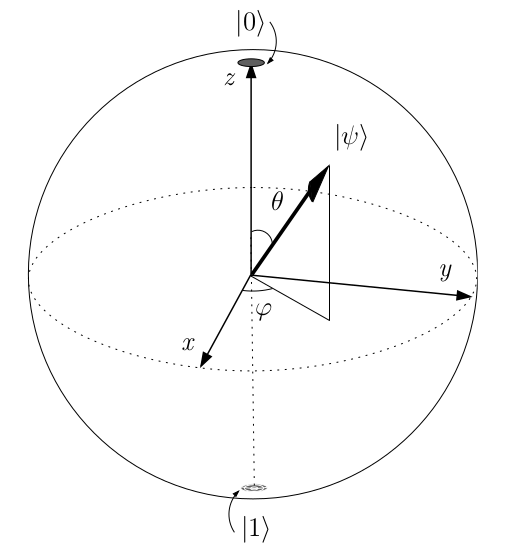
\includegraphics[width=5cm]{Figures/bloch}
	\caption{Bloch sphere \cite{portugal}.}
\end{figure}

\paragraph{Measurements.} It is a probabilistic operation that allows one to recover some classical information. The measurement of $|\psi\rangle = \alpha|0\rangle + \beta|1\rangle$ returns $|0\rangle$ with probability $|\alpha|^2$ and $|1\rangle$ with probability $|\beta|^2$. It also alters the state of a qubit and forces it to collapse to state $|0\rangle$ or $|1\rangle$, respectively. In this case, we say the measurement was done against the computational basis $\{|0\rangle,|1\rangle\}$.

\paragraph{Unitary operations.}  The temporal evolution of an isolated quantum system is described by linear transformations, represented by matrices. Transformations that map unitary vector onto unitary vectors are called \textit{unitary transformations} $U$ and can be defined by the following property:
$$ U^{\dagger}U = UU^{\dagger} = I, $$
where $U^{\dagger} = \left(\overline{U}\right)^T$ is the adjoint matrix and $I$ is the identity. These are reversible operations. 

Some usual gates are NOT, Hadamard, phase-shift and phase-flip:

\begin{itemize}
	\item NOT
	$$ N = \begin{pmatrix}
	0 & 1\\
	1 & 0
	\end{pmatrix} $$
	\item Hadamard
	$$ H = \frac{1}{\sqrt{2}}\begin{pmatrix}
	1 & 1\\
	1 & -1
	\end{pmatrix} $$
	\item Phase-shift
	$$ V_\theta = \begin{pmatrix}
	1 & 0\\
	0 & e^{i\theta}
	\end{pmatrix} $$
	\item Phase-flip\footnote{Note that, in fact, $Z=V_\pi$.}
	$$ Z = \begin{pmatrix}
	1 & 0\\
	0 & -1
	\end{pmatrix} $$
\end{itemize}

\paragraph{Tensor product.} The tensor product between two states
$$|\psi\rangle = \begin{pmatrix}
\psi_1\\
\vdots\\
\psi_m
\end{pmatrix}
\text{ and }
|\varphi\rangle = \begin{pmatrix}
\varphi_1\\
\vdots\\
\varphi_p
\end{pmatrix}$$
is computed as
$$
|\psi\rangle \otimes |\varphi\rangle = 
\begin{pmatrix}
\psi_1\varphi_1\\
\vdots\\
\psi_1\varphi_p\\
\psi_2\varphi_1\\
\vdots\\
\psi_2\varphi_p\\
\vdots\\
\psi_m\varphi_1\\
\vdots\\
\psi_m\varphi_p\\
\end{pmatrix}.
$$

In general, given two matrices $A\in\mathbb{C}^{m \times n}$ and $B\in\mathbb{C}^{p \times q}$, the tensor product is the matrix $A\otimes B\in\mathbb{C}^{mp \times nq}$ given by
$$ A\otimes B = \begin{pmatrix}
a_{11}B & a_{12}B & \cdots & a_{1n}B\\
a_{21}B & a_{22}B & \cdots & a_{2n}B\\
\vdots & \vdots & \ddots & \vdots\\
a_{m1}B & a_{m2}B & \cdots & a_{mn}B\\
\end{pmatrix} $$
where $a_{ij}$ is the $(i,j)$-element of $A$.

Given two linear transformations $A$ and $B$, we can define a new linear mapping by
$$ (A \otimes B)(|u\rangle \otimes |v\rangle) = A|u\rangle \otimes B|v\rangle. $$

Notation:
\begin{itemize}
	\item We can indistinguishably write $|\psi\rangle \otimes |\varphi\rangle = |\psi\rangle|\varphi\rangle = |\psi,\varphi\rangle = |\psi\varphi\rangle$.
	\item $|\psi\rangle^{\otimes n} = \underbrace{|\psi\rangle \otimes \cdots |\psi\rangle}_{n \text{ times}}$ and $A^{\otimes n} = \underbrace{A \otimes \cdots A}_{n \text{ times}}$.
\end{itemize}


\paragraph{Two or more qubits systems.} The state of a 2-qubit is an element of the tensor product space $\mathbb{C}^4 = \mathbb{C}^2 \otimes \mathbb{C}^2$, which is spanned by
$$|00\rangle = \begin{pmatrix}1\\0\\0\\0\end{pmatrix},\quad |10\rangle = \begin{pmatrix}0\\1\\0\\0\end{pmatrix},\quad |01\rangle = \begin{pmatrix}0\\0\\1\\0\end{pmatrix},\quad |11\rangle = \begin{pmatrix}0\\0\\0\\1\end{pmatrix}.$$

A generic state of 2 qubits it therefore of the form
$$ |\psi\rangle = \alpha|00\rangle + \beta|01\rangle + \gamma|10\rangle + \delta|11\rangle $$
with $|\alpha|^2+|\beta|^2+|\gamma|^2+|\delta|^2=1$.

In general, writing states as the decimal number correspoding to the binary representation (e.g. $|11\rangle \rightarrow |3\rangle$), a $n$-qubit state is described as
$$ |\psi\rangle = \sum_{i=0}^{2^n-1}\alpha_i|i\rangle, \text{ with } \sum_{i=0}^{2^n-1}|\alpha_i|^2=1. $$

As a generalisation of the 1-qubit case, the measurement of a $n$-qubit state changes it and forces it to collapse to one of the possible $|i\rangle$ states, each of which is measured with probability $|\alpha_i|^2$.

Among unitary operations available to 2-qubits states, we have the swap gate $X$ and the control-not gate $N_C$:
$$ X = \begin{pmatrix}
1 & 0 & 0 & 0\\
0 & 0 & 1 & 0\\
0 & 1 & 0 & 0\\
0 & 0 & 0 & 1\\
\end{pmatrix},\quad
N_C = \begin{pmatrix}
1 & 0 & 0 & 0\\
0 & 1 & 0 & 0\\
0 & 0 & 0 & 1\\
0 & 0 & 1 & 0\\
\end{pmatrix}. $$

The control-not gate changes the state of the second qubit only if the first qubit is in the state $|1\rangle$. It implements the mapping $|xy\rangle \mapsto |x\rangle \otimes |x\oplus y\rangle$.

The Toffoli gate acts on 3 qubits and is a ``control-control-not'': it implements the function $|xyz\rangle \mapsto |xy\rangle \otimes |z\oplus xy\rangle$, i.e., it changes the state of the last qubit if the two first qubits are in state $|11\rangle$.

\paragraph{Quantum entanglement.} Consider the states $|\psi\rangle = a|0\rangle + b|1\rangle$ and $|\varphi\rangle = c|0\rangle + d|1\rangle$. Their tensor product is $|\psi\varphi\rangle = ac|00\rangle + ad|01\rangle + bc|10\rangle + bd|11\rangle$. It turns out that a general state is not on this form, unless it has $\alpha\delta = \beta\gamma$.

We say a quantum state is \textit{entangled} when it cannot be written as a tensor product of two other states. For example, $\frac{1}{\sqrt{2}}(|00\rangle+|11\rangle)$ cannot have such a decomposition, and hence is an entangled state.

\paragraph{Quantum circuits} Quantum circuits are graphical representations of a procedure, i.e., a sequence of logical operations performed on a system. Unlike classical circuits, the wires must not be regarded as physical connections and their components are not available ``on the shelf''.

\begin{figure}[h!]
	\centering
	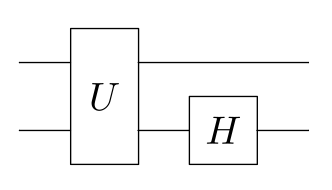
\includegraphics[width=4cm]{Figures/circuit}
	\caption{Example of quantum circuit representing $|\psi\rangle \mapsto (I\otimes H)(U|\psi\rangle)$ \cite{valiron}.}
\end{figure}

\section{Shor's algorithm}

The advantage of quantum algorithms over classical ones appears when using some quantum property such as entanglement or the interference, brought by complex coefficients.

In fact, quantum algorithms are based on a few ``real'' quantum constructions, such as quantum Fourier transform, quantum walk and amplitude amplification. The rest is composed of classical analysis and possibly an \textit{oracle}: a quantum circuit corresponding to a reversible operation.

Some interesting problems in algebra and number theory reduce to the problem of order finding. For example, the problem of factorising an integer number, which is addressed by Shor's algorithm \cite{shor}.

\paragraph{Factorisation.} The objective of the \textit{factorisation problem} is to factorise a big number $N$ into prime numbers. Note that at least $n=\lceil\log_2N\rceil$ qubits are needed to store $N$ and that $n$ is the maximum number of prime factors. We will show how this problem reduces to the problem of finding the order of a randomly generated integer $x<N$ generated randomly.

If $N$ is even, 2 is trivially a factor. In addition, if $x$ and $N$ have common factors, then $\gcd(x,N)$ gives a factor of $N$; so we focus on investigating the case when $x$ and $N$ are coprimes.

\begin{definition}
	The order of $x$ modulo $N$ is the least positive integer $r$ such that
	$$ x^r \equiv 1 \mod N. $$
\end{definition}

\begin{theorem}[Euler's Theorem]
	If $x$ and $N$ are coprime positive integers, then
	$$ x^{\varphi(N)} \equiv 1 \mod N, $$
	where $\varphi(N)$ is the Euler's totient function, i.e., it indicates the number of coprimes to $N$ which are less or equal to it.
\end{theorem}

The \textit{order finding problem} is to find $r$, given $x$ and $N$ coprimes. The algorithm is built up on the following two theorems.

\begin{theorem}
	Let $N$ be a composite number stored with $n$ qubits and $x$ be non-trivial solution of the equation $x^2 \equiv 1 \mod N$ in the range $1 \le x \le N$, i.e., $x \not\equiv \pm 1 \mod N$. Then at least one of $\gcd(x+1,N)$ and $\gcd(x-1,N)$ is a non-trivial factor of $N$.
\end{theorem}

\begin{proof}
	Note that $x^2 \equiv 1 \mod N \Leftrightarrow x^2-1 \equiv 0 \mod N \Leftrightarrow (x+1)(x-1) \equiv 0 \mod N$, which means that $N$ is a divisor of $(x+1)(x-1)$. If $1<x<N-1$, then $0<x-1<x+1<N$ and $N$ cannot be a divisor of $(x+1)$ neither of $(x-1)$ separately. So both $(y+1)$ and $(y-1)$ must have factors of $N$. In this case, at least one of $\gcd(y+1,N)$ and $\gcd(y-1,N)$ produce a non-trivial factor of $N$\footnote{Such factor can be computed by using Euclid's algorithm.}.
\end{proof}

\begin{theorem}
	Suppose $N = p_{1}^{\alpha_1}...p_{m}^{\alpha_m}$ is the prime factorisation of and odd composite positive integer. Let $x$ be an integer chose uniformly at random such that $1 \le x\le N-1$ and $\gcd(x,N)=1$. Let $r$ be the order of $x$ modulo $N$. Then
	$$ \mathrm{Pr}\{\text{$r$ is even and $x^{r/2}\not\equiv\pm1\mod N$}\} \ge 1-\frac{1}{2^m}. $$
\end{theorem}

\begin{proof}
	See \cite{ekert}, pp. 751-752\footnote{Actually, these authors use a slightly different bound for the probability: $1-1/2^{m-1}$.}.
\end{proof}

The algorithm runs as follows.

\begin{algorithm}[h!]
	\caption{Shor's algorithm for factorising $N$.}
	If $N$ is even, return the factor 2.\\
	Randomly choose $x$ such that $1 \le x \le N-1$.\\
	If $\gcd(x,N)\neq1$, return the factor $\gcd(x,N)$.\\
	Find the order $r$ of $x$ modulo $N$.\\
	If $r$ is even and $x^{r/2}\not\equiv\pm 1\mod N$, then $\gcd(x^{r/2}+1)$ and $\gcd(x^{r/2}-1)$ are non-trivial factors.\\
	Else, restart the algorithm.
\end{algorithm}

Some remarks:

\begin{itemize}
	\item The method fails if $N$ is the power of a prime number. But in this case there exists a a classical algorithm to solve the problem \cite{portugal}. %Which one?
	\item The problem is finding the order of $x$ modulo $N$, for which there is no efficient classical procedure available. This problem is addressed in the next part.
\end{itemize}

\paragraph{Order finding.} The problem of order finding, i.e., given $x$ and $N$ coprimes, to find $r$ such that $x^r \equiv 1 \mod N$ is related to the matrix eigendecomposition. A unitary $U$, being a Hermitian matrix, can be decomposed as
$$ U=\sum_j \lambda_ju_ju_j^\dagger, $$
where $u_j$ are orthonormal eigenvectors and $\lambda_j$ are the associated eigenvalues.

Let us assume that $N=2^n$ and consider the operation $U_a$ on $n$ qubits that implements the mapping
$$U : \quad |j\rangle \mapsto |j\cdot x\mod N\rangle.$$
The operator is unitary because $x$ and $N$ are coprimes and the image of $\{0,...,N-1\}$ is the whole set. In particular, $U^k$ sends $|j\rangle \mapsto |j\cdot x^k \mod N\rangle$, so if $x^r \equiv 1 \mod N$, the map $U^r$ is the identity map.

The eigenstates of $U$ are of the form
$$ |u_s\rangle = \frac{1}{\sqrt{r}} \sum_{k=0}^{r-1}\exp{\left(-\frac{2\pi i sk}{r}\right)}|x^k \mod N \rangle $$
for $0 \le s \le r-1$. The eigenvalues are the $r$-th roots of the unity, having the form $e^{2\pi is/r}$, since
$$ U|u_s\rangle = \exp\left(\frac{2\pi is}{r}\right)|u_s\rangle. $$

An algorithm for finding such eigenvalues should be enough to find the order $r$ of $x$ modulo $N$\footnote{An alternative unitary could have been used: $V|j\rangle|k\rangle=|j\rangle|k+x^j\mod N\rangle$.}.

\paragraph{Quantum Fourier transform.} The Fourier transform is an operation that can be performed faster in quantum computers. The quantum Fourier transform (QFT) \cite{griffighs} is defined in analogy with the discrete Fourier transform. It is the linear mapping:
\begin{align*}
	\hat{f}\ :\ \mathbb{C}^N &\rightarrow \mathbb{C}^N\\
	|j\rangle &\mapsto \frac{1}{\sqrt{N}}\sum_{k=0}^{N-1}e^{2\pi ijk/N}|k\rangle
\end{align*}

Let us consider $N=2^n$ with orthonormal basis $\{|0\rangle,\dots,|2^n-1\rangle\}$. We shall use the \textit{binary representation} $j =: j_1j_2\dots j_n$ to represent $j = \sum_{i=1}^{n}j_{i}2^{n-i}$ and the \textit{binary fraction} $j =: 0.j_1j_2\dots j_n$ to represent $j = \sum_{i=1}^{n}j_{i}2^{-i}$.

It will be useful to consider an alternative form of the QFT which is indeed so important that could be considered its definition itself:

$$ |j_1\dots j_n\rangle \mapsto \frac{\left(|0\rangle+e^{2\pi i0.j_n}|1\rangle\right)\otimes\left(|0\rangle+e^{2\pi i0.j_{n-1}j_n}|1\rangle\right)\otimes\dots\otimes\left(|0\rangle+e^{2\pi i0.j_1\dots j_n}|1\rangle\right)}{2^{n/2}}. $$

The equivalence between the two expressions can be shown as follows \cite{nielsen}:

\begin{align*}
	&\frac{1}{2^{n/2}}\sum_{k=0}^{2^n-1}e^{2\pi ijk/2^n}|k\rangle\\
	=\ &\frac{1}{2^{n/2}}\sum_{k_1=0}^{1}\dots\sum_{k_n=0}^{1}e^{2\pi ij(\sum_{l=1}^{n}k_l/2^{l})}|k_1\dots k_n\rangle \ &\text{(write in binary representation)}\\
	=\ &\frac{1}{2^{n/2}}\sum_{k_1=0}^{1}\dots\sum_{k_n=0}^{1}\prod_{l=1}^{n}\otimes e^{2\pi ijk_l/2^l}|k_l\rangle\ &\text{(tensor product decomposition)}\\
	=\ &\frac{1}{2^{n/2}}\prod_{l=1}^{n}\otimes\left( \sum_{k_l=0}^{1} e^{2\pi ijk_l/2^l}|k_l\rangle \right)\ &\text{(factorise the binary powers)}\\
	=\ &\frac{1}{2^{n/2}}\prod_{l=1}^{n}\otimes\left( |0\rangle + e^{2\pi ij/2^l} |1\rangle \right).
\end{align*}

The product representation allows one to implement the quantum circuit for the QFT using Hadamard and $R_k$ rotation gates, the latter being of the form\footnote{The attentive reader will notice that $R_k = V_{2\pi/2^k}$.}
$$ R_k := \begin{pmatrix}1 & 0\\ 0 & e^{2\pi i/2^k}\end{pmatrix}. $$

\begin{figure}[h!]
	\centering
	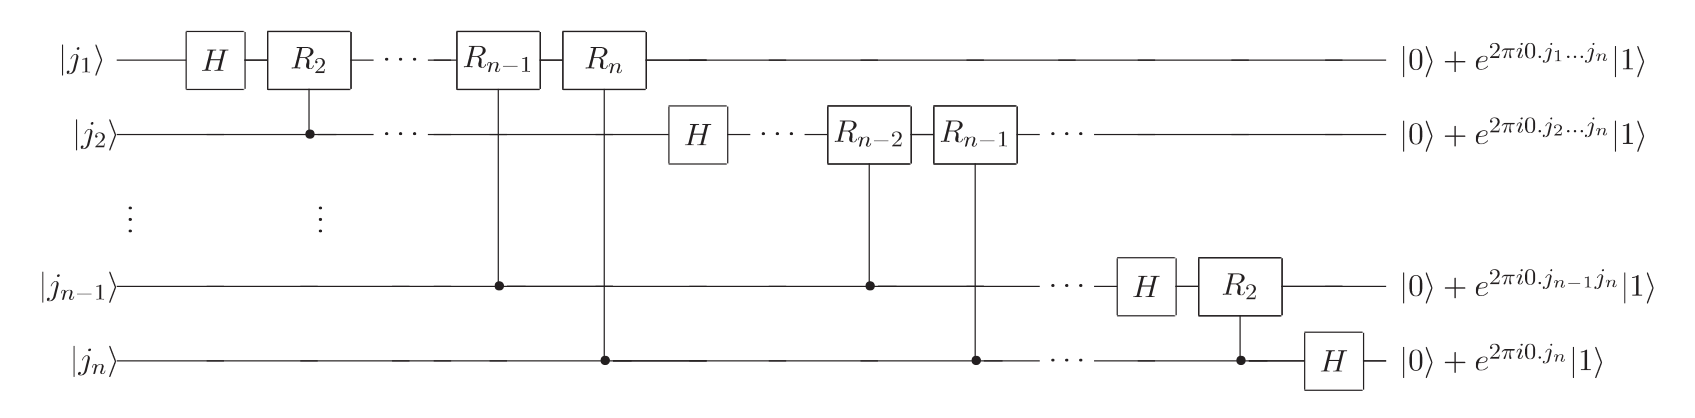
\includegraphics[width=12cm]{Figures/qft-circuit}
	\caption{Quantum circuit that implements the QFT \cite{nielsen}.}
	\label{fig-qft}
\end{figure}

To conclude this section, we remark that the QFT, as a linear operation, may be written in matrix form\cite{wiki}:

$$ F_N = \frac{1}{\sqrt{N}}
	\begin{pmatrix}
	1 & 1 & 1 & 1 & \cdots & 1 \\
	1 & \omega_n & \omega_n^2 & \omega_n^3 & \cdots & \omega_n^{N-1} \\
	1&\omega_n^2&\omega_n^4&\omega_n^6&\cdots&\omega_n^{2(N-1)}\\ 1&\omega_n^3&\omega_n^6&\omega_n^9&\cdots&\omega_n^{3(N-1)}\\
	\vdots&\vdots&\vdots&\vdots&&\vdots\\
	1&\omega_n^{N-1}&\omega_n^{2(N-1)}&\omega_n^{3(N-1)}&\cdots&\omega_n^{(N-1)(N-1)}
	\end{pmatrix}
$$
where $N=2^n$ and $\omega_n:=e^{2\pi i/2^n}$. This allows one to verify that $F_NF_N^{\dagger} = I = F_N^{\dagger}F_N$, therefore concluding that the Fourier transform is a unitary transformation.

\paragraph{Quantum phase estimation.} Suppose a unitary operator $U$ has an eigenvector $|u\rangle$ with eigenvalue $e^{2\pi i\varphi}$, where $\varphi$ is unknown. The objective of the \textit{phase estimation subroutine} is to estimate the value of $\varphi$. We assume we have oracles capable of preparing the state $|u\rangle$ and performing controlled-$U^{2^j}$ operations.

The procedure uses two registers: the first contains $t$ qubits initially in state $|0\rangle$. The number $t$ depends on the desired accuracy for $\varphi$ and on the probability we want the procedure to be successful. The second register begins with the state $|u\rangle$ and contains as many qubits as necessary to store it.

The first step is to apply the following circuit to the registers.

\begin{figure}[h!]
	\centering
	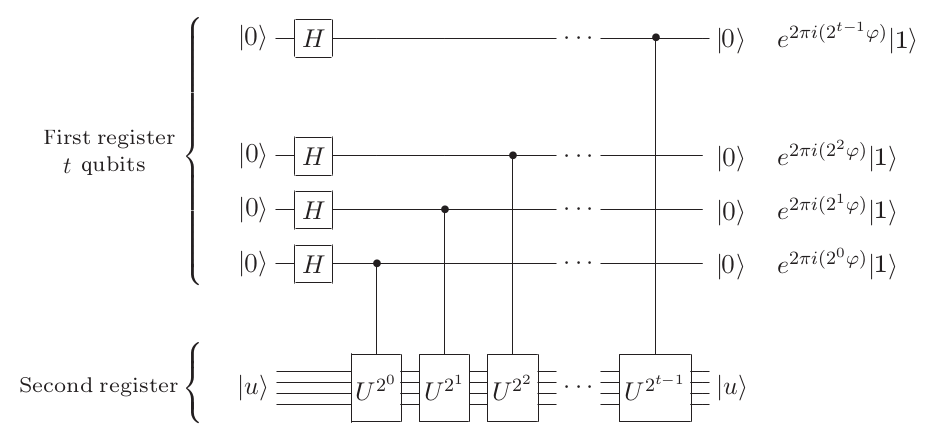
\includegraphics[width=10cm]{Figures/phase-estimation-1}
	\caption{Quantum circuit for first step of phase estimation (normalisation has been omitted on the right side) \cite{nielsen} .}
\end{figure}

The final state of the first register is
\begin{align*}
	&\frac{1}{2^{t/2}}\left(|0\rangle+e^{2\pi i2^{t-1}\varphi}|1\rangle\right)\left(|0\rangle+e^{2\pi i2^{t-2}\varphi}|1\rangle\right) \dots \left(|0\rangle+e^{2\pi i2^{0}\varphi}|1\rangle\right)\\
	=\ &\frac{1}{2^{t/2}}\sum_{k=0}^{2^t-1}e^{2\pi i\varphi k}|k\rangle.
\end{align*}

The second step is to apply the inverse Fourier transform on the first register\footnote{To do so, we just have to inverse the circuit for QFT on Figure \ref{fig-qft}.} and the third step is to measure it. Note that, if we write the previous expression using the binary fraction representation, we have
$$ \frac{1}{2^{t/2}}\left(|0\rangle+e^{2\pi i0.\varphi_t}|1\rangle\right)\left(|0\rangle+e^{2\pi i0.\varphi_{t-1}\varphi_{t}}|1\rangle\right) \dots \left(|0\rangle+e^{2\pi i0.\varphi_1...\varphi_t}|1\rangle\right). $$
Comparing it with the (product) expression for the Fourier transform, one can see that the result of applying the inverse Fourier transform is the state $|\varphi_1\dots\varphi_r\rangle$ and a measurement in the computational basis gives exactly an estimation for $\varphi$!

\begin{figure}[h!]
	\centering
	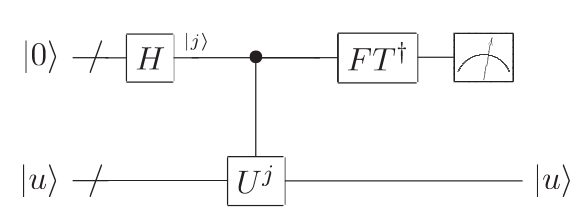
\includegraphics[width=6cm]{Figures/phase-estimation-2}
	\caption{Schematic of the overall phase estimation subroutine \cite{nielsen} .}
\end{figure}

Summarising, the phase estimation subroutine gives an estimation $\tilde{\varphi}$ to the phase of an eigenvalue of a unitary $U$, which is precisely what we wanted to implement the order finding algorithm. The inverse Fourier transform performs
$$ \frac{1}{2^{t/2}}\sum_{j=0}^{2^{t-1}}e^{2\pi i\varphi j}|j\rangle|u\rangle \mapsto |\tilde{\varphi}\rangle|u\rangle. $$

\begin{theorem}[Accuracy of $\varphi$ \cite{nielsen}, pp. 223-224]
	To successfully obtain $\varphi$ accurate to $n$ bits with probability of success at least $1-\epsilon$, we choose
	$$ t = n + \left\lceil \log\left(2+\frac{1}{2\epsilon}\right) \right\rceil. $$
\end{theorem}

\paragraph{Continued fraction expansion.} Let us recapitulate what we have so far: we have reduced the factorisation problem to the order finding problem, which can be solved by calculating eigenvalues of a unitary $U$ of the form $e^{2\pi is/r}$. The quantum phase estimation procedure uses the QFT to estimate the phase $\varphi$ of an eigenvalue $e^{2\pi i\varphi}$. So we have an estimation
$$ \tilde{\varphi} \approx \frac{s}{r}. $$

It misses one building block in order to solve our problem: how to retrieve $r$ from $\tilde{\varphi}$. To do so, we shall use \textit{continued fraction expansions}. The results on this topic can be deepened in \cite{hardy}. 

\begin{definition}
	A finite simple continued fraction is an expression of the form
	$$ a_0 + \dfrac{1}{a_1 + \dfrac{1}{a_2 + \dfrac{1}{\ddots+\dfrac{1}{a_N}}}} $$
	which is denoted by $[a_0,  a_1, a_2, \cdots, a_N]$, with $a_i \in \mathbb{N}^*\ \forall i\in \llbracket 1, N\rrbracket$.\\
	We define the $n$-th convergent to this continued fraction as $[a_0,\dots,a_n]$ for $0\le n \le N$.
\end{definition}

\begin{theorem}
	The $n$-th convergent may be written as a fraction
	$$[a_0,\dots,a_n]=\frac{p_n}{q_n}$$
	whose coefficients are given by the following recurrence relation:
	$$
	\begin{array}{ll}
		p_0:=a_0\\
		q_0:=1
	\end{array}\quad
	\begin{array}{ll}
		p_1:=a_1a_0+1\\
		q_1:=a
	\end{array}\quad
	\begin{array}{ll}
		p_n:=a_np_{n-1}+p_{n-2}\\
		q_n:=a_nq_{n-1}+q_{n-2}
	\end{array}\ (2\le n \le N).
	$$
\end{theorem}

\begin{proof}
	See \cite{hardy}, pp. 166-167.
\end{proof}

The next two theorems will present the \textit{continued fractions algorithm} to approximate $\tilde{\varphi}$ by a $n$-th convergent and explain why it suffices to solve our problem.

\begin{theorem}[Continued fraction algorithm]
	Any rational number $x$ can be represented by a finite simple continued fraction $[a_0,\dots,a_N]$.\\
\end{theorem}

\begin{proof}
	See \cite{hardy}, pp. 173-174.
\end{proof}

The algorithm runs as follows.

\begin{algorithm}[h!]
	\caption{Continued fraction algorithm for rational $x$.}
	Set $a_0 = \lfloor x \rfloor$. Then $x=a_0+\xi_0$, with $\xi_0\in[0,1[$.\\
	While $\xi_i \neq 0$: $a_{i+1}=\lfloor1/\xi_{i}\rfloor$ and $1/\xi_{i}=a_{i+1}+\xi_{i+1}$, with $\xi_{i+1}\in[0,1[$.\\
	The continued fraction is $[a_0,\dots,a_N]$, where $N$ is such that $\xi_N=0$.
\end{algorithm}

\begin{theorem}
	Suppose $s/r$ is a rational number such that
	$$ \left|\frac{s}{r}-\varphi\right| \le \frac{1}{2r^2}.$$
	Then $s/r$ is a convergent of the continued fraction for $\varphi$.
\end{theorem}

\begin{proof}
	See \cite{hardy}, pp. 196-197.
\end{proof}

Since $\tilde{\varphi}$ is an approximation of $s/r$ accurate to $n=\lceil\log_2N\rceil$ qubits, the theorem applies. Summarising, given $\tilde{\varphi}$, we can use the continued fraction algorithm to find an irreducible fraction $s'/r'=s/r$. Then, $r'$ is our candidate for the order. We check calculating $x^{r'} \mod N$; if the result is $1$, we are done!

\section{Circuit implementation}

Now that we know the quantum algorithm to factorise a number, we can devote our attention to the implementation in terms of quantum circuit. Although we have already provided a circuit for the QFT, the oracle remains a mysterious black box.

TO DO: use \cite{draper, beauregard}.

\section{Implementation}

The implementations was be made using \textit{ProjectQ} \cite{projectq, steiger}.

TO DO

\newpage

\begin{thebibliography}{10}

\bibitem{valiron} Valiron, B. ``Quantum computation: a tutorial''. \textit{New Generation Computing}, vol. 30, no. 4, pp. 271-296, oct. 2012.

\bibitem{portugal} Portugal, R. et al. \textit{Uma introdu��o � computa��o qu�ntica}. S�o Carlos: SBMAC, 2004.

\bibitem{nielsen} Nielsen, Michael A and Chuang, Isaac L. \textit{Quantum computation and quantum information}. 10th anniversary edition. Cambridge: Cambridge University Press, 2010.

\bibitem{shor} Shor, Peter. ``Polynomial-Time Algorithms for Prime Factorization and Discrete Logarithms on a Quantum Computer''. \textit{SIAM Journal on Computing}, vol. 26, no. 5, pp. 1484-1509, 1997.

\bibitem{ekert} Ekert, A. and Jozsa, R. ``Quantum computation and Shor's factoring algorithm''. \textit{Reviews of Modern Physics}, vol. 68, no. 3, pp. 733-753, 1996.

\bibitem{griffighs} Griffiths, Robert B. and Niu, Chi-Sheng. ``Semiclassical Fourier Transform for Quantum Computation''. \textit{Physycal Review Letters}, vol. 76, no. 17, pp. 3228-3231, 1996.

\bibitem{wiki} Wikipedia. \textit{Quantum Fourier transform}. Available in: \url{https://en.wikipedia.org/wiki/Quantum_Fourier_transform}. Access on: 18 dec. 2018.

\bibitem{hardy} Hardy, G. H. and E. M. Wright. \textit{An introduction to the
theory of numbers}. 6th edition. Oxford : Oxford University Press, 2008.

\bibitem{draper} Draper, Thomas G. \textit{Addition on a quantum computer}. Available in: \url{https://arxiv.org/abs/quant-ph/0008033}. Access on: 14 dec. 2018.

\bibitem{beauregard} Beauregard, Stephane. ``Circuit for Shor's algorithm using $2n+3$ qubits''. \textit{Quantum Information and Computation}, vol. 3, no. 2 (2003) pp. 175-185.

\bibitem{projectq} ProjectQ. Availabe in: \url{https://projectq.ch/}. Access on: 28 nov. 2018.

\bibitem{steiger} Steiger, Damian S.; H�ner, Thomas and Troyer, Matthias. ``ProjectQ: an open source software framework for quantum computing''. \textit{Quantum}, vol. 2, p. 49, jan. 2018.


\end{thebibliography}

\end{document}